\chapter{In- and output}
\section{The input file - *.json}
In the following we will describe the input parameters of IFOS3D. The verbatim text shows, how they appear in \textit{in\_and\_out/ifos3d\_inv\_all\_parameters.json}. There is also a commented json file: \textit{in\_and\_out/ifos3d\_inv\_all\_parameters\_commented.json}. The parameters used for the wavefield simulation mostly resemble the parameters of SOFI3D and are also described in the SOFI manual.
\subsection{The grid and its decomposition}
\subsubsection*{The grid}
\begin{verbatim}
"Note that y denotes the vertical direction !" : "comment",
"3-D Grid" : "comment",
			"NX" : "160",
			"NY" : "184",
			"NZ" : "160",
			"DX" : "0.8",
			"DY" : "0.8",
			"DZ" : "0.8",
\end{verbatim}
The cartesian grid system is specified by the number of grid points in each direction (\textbf{NX, NY, NZ}) and by the distance between grid points \textbf{DX, DY, DZ} chosen in the input file. Hereby \textbf{NY} and \textbf{DY} denote the vertical direction! 
The grid spacing needs to satisfy the dispersion criterion at least up to the maximum frequency and minimum wavelength used in the inversion. In case the dispersion criterion is violated for the frequency range of the source wavelet, a warning is given at the beginning of the simulation. The dispersion criterions are given in the SOFI3D manual.
\subsubsection*{Domain decomposition}
\begin{verbatim}
"Domain Decomposition" : "comment",
			"NPROCX" : "2",
			"NPROCY" : "2",
			"NPROCZ" : "2",
\end{verbatim}


The parallelisation is based on domain decomposition. Each processor performs the FWI algorithm for a small subvolume of the total grid system. \textbf{NPROCX}, \textbf{NPROCY} and \textbf{NPROCZ} define the number of processors in each direction, which gives a total number of $NPROCX\times NPROCY\times NPROCZ$ processors. Note, that the number of processors in each direction needs to be a common factor of the number of grid points in this direction.

\subsection{FD-modeling parameters}
\subsubsection*{Order of FD operator}
\begin{verbatim}
"FD order" : "comment",
			"FDORDER" : "4",
			"FDCOEFF" : "2",
\end{verbatim}

The order of the spatial FD-sheme,  which is used for the stress and velocity updates can be chosen as \textbf{FDORDER}=2, 4, 6, 8, 10, and 12. 
These orders result in different dispersion and stability criterions (section~\ref{sec:SOFI3Dcharacter}). A larger FD-order enables a larger grid spacing, however in case of strong heterogeneities a smaller FD-operatot is more accurate. 
With the option \textbf{FDCOEFF} the user can switch between Taylor (\textbf{FDCOEFF}=1) and Holberg (\textbf{FDCOEFF}=2) FD coefficients. Within the CPML boundary a fourth order operator is applied automatically. 
We also use fourth order operators to calculate the spatial derivatives of the wavefield velocity, which are needed for the gradient calculation. IFOS3D uses a second order time discretisation.
\subsubsection*{Time Stepping}
\begin{verbatim}
"Time Stepping" : "comment",
			"TIME" : "0.06",
			"DT" : "5.0e-05",
\end{verbatim}

\textbf{TIME} defines the total simulation length.  The time stepping \textbf{DT} must be chosen to satisfy the stability criterion (SOFI3D  maunual) and thus depends on the grid spacing and the maximum velocity. 
In case of violation IFOS3D will give a warning and terminate. The number of timesteps of the inversion is given by $TIME/DT$.

\subsection{Sources}
\begin{verbatim}
"Source" : "comment",
			"SOURCE_SHAPE" : "4",
			"SOURCE_TYPE" : "4",
			"ALPHA" : "45.0",
			"BETA" : "45.0",
			"SIGNAL_FILE" : "./STF/stf.su",
			"SRCREC" : "1",
			"SOURCE_FILE" : "./sources/sources_toy.dat",
			"RUN_MULTIPLE_SHOTS" : "1",
\end{verbatim}

\subsubsection*{The wavelet}
Different wavelets for the modeling can be chosen:
\begin{itemize}
 \item \textbf{SOURCE\_SHAPE}=1: Ricker wavelet:\\ $s=(1.0-2.0\tau ^2)\text{exp}(-\tau ^2); \hspace{0.5cm}	\tau=\pi f_c(t-1.5/f_c-t_d);$	
\item \textbf{SOURCE\_SHAPE}=2: Fuchs-M\"uller wavelet:\\ $s(t)=\text{sin}(2.0\pi (t-t_d)f_c-0.5 \text{sin}(4.0\pi (t-t_d)f_c); \hspace{0.2cm}\text{for}\hspace{0.2cm}(t_d<t<t_d+1/f_c) \hspace{0.4cm}\text{else}\hspace{0.2cm} s(t)=0$
\item \textbf{SOURCE\_SHAPE}=4: sin$^3$-wavelet:\\ $s(t)=0.75\pi f_c\text{sin}(\pi f_c(t-t_d)^3;\hspace{0.2cm}\text{for}\hspace{0.2cm}(t_d<t<t_d+1/f_c) \hspace{0.5cm}\text{else}\hspace{0.2cm} s(t)=0$
\item \textbf{SOURCE\_SHAPE}=5: step function:\\ $s(t)=0.0; \hspace{0.2cm}\text{if}\hspace{0.2cm}(t<t_d) \hspace{0.5cm}\text{else} \hspace{0.2cm} s(t)=1.0; $
\end{itemize}
The employed center frequency $f_c$ and the time delay of the source wavelet $t_d$ are defined in the source file. An exemplary plot of the different wavelets and the corresponding spectra can be seen in the SOFI3D manual. 
Note, that the symmetric Ricker wavelet is delayed and its maximum period is excited at the source location after one period. The step function is used for the calculation of the diagonal Hessian approximation. \\
If you want to define your own wavelet, you can include this either in the source code in \textit{src/wavelet.c} or use \textbf{SOURCE\_SHAPE}=3 and read in an external wavelet from \textbf{SIGNAL\_FILE}. 
This file should contain the source signal in ASCII with the correct time sampling and with one sample per line, like \\
----------------\\
0.0\\
0.01\\
0.03\\
...\\
----------------
\subsubsection*{The source type}
You can either choose an explosive source (\textbf{SOURCE\_TYPE}=1) exciting compressional waves or a  point force directed in $x$, $y$ (vertical) or $z$  (\textbf{SOURCE\_TYPE}=2,3,4) direction. With \textbf{SOURCE\_TYPE}=5 it is also possible to define a force in arbitrary direction by using the angles \textbf{ALPHA} and \textbf{BETA}. This is illustrated in the SOFI manual. 
The plane wave excitation (\textbf{SOURCE\_REC}=2) was not yet tested for inversion in IFOS3D but can also be chosen here.
%# Plane wave excitation,if PLANE_WAVE_DEPTH>0, SRCREC is treated as 0
%depth_of_plane_wave_excitation_(no<=0)_(in_meter)_(PLANE_WAVE_DEPTH) = 0.0
%dip_of_plane_wave_from_vertical_(in_degrees)_(PHI) =0.0
%duration_of_source-signal_(in_seconds)_(TS) = 0.0033
\subsubsection*{The source location}
The source locations are defined in the \textbf{SOURCE\_FILE} located in the folder \textit{sources}. For each source the parameters XSRC, YSRC and ZSRC are defined, which are the $x$-, $y$- and $z$-coordinates of the source position in meter. Additionally a time delay TD in seconds, a center frequency of the source signal (FC) in Hz and an amplitude of the source signal are chosen. An example file for a source located at (XSRC=100m, YSRC=50m and ZSRC=2m) with a center frequency of 20Hz and no time delay looks like:\\
----------------\\
100.0 \hspace{0.2cm} 50.0 \hspace{0.2cm} 2.0 \hspace{0.2cm} 0.0 \hspace{0.2cm} 20.0 \hspace{0.2cm} 1.0\\
----------------
\subsection{The model}
\subsubsection*{Model input}
\begin{verbatim}
"Model" : "comment",
			"READMOD" : "0",
			"MFILE" : "model/toy",
\end{verbatim}

The elastic subsurface model is parametrised by the compressional wave velocity $v_p$, the shear wave velocity $v_s$ and the density $\rho$ at each grid point. Model parameters are required for the forward modeling and as starting model for the inversion. There are two options to read in the model parameters:\\
\textbf{READMOD}=1: The model parameters of an external model are read in from the model files defined as \textbf{MFILE}, here for example  \textit{toy.$v_p$}, \textit{toy.$v_s$} and \textit{toy.$\text{rho}$} placed in the folder \textit{par/model}. In these files, each material parameter value must be saved as 32 bit (4 byte) native float.
Velocities must be in m/s, density values in kg/m$^3$ defined at each grid point. The values are read in with \textit{src/readmod.c} and you may look at this source code for the correct order of parameters.\\
\textbf{READMOD}=0: It is also possible to generate the model parameters in the program on the fly. The corresponding C-function, e.g. \textit{src/hh.c} is included in the \textit{src/Makefile}. 
\subsubsection*{Viscoelasticity}
\begin{verbatim}
"Q-approximation" : "comment",
			"L" : "0",
			"FL1" : "1000.0", 
			"TAU" : "0.000001",
\end{verbatim}

The inversion code was only tested in the elastic version (\textbf{L}=0). However, the viscoelasic version of SOFI3D is included in the package and can be used for forward modeling. In this case, the elastic update functions for the velocities need to be replaced by the viscoelastic update functions available in \textit{src}. No inversion code is  included for viscoelastic parameters and they can be only used as passive parameters. For further information on viscoelasticity please look in the SOFI manual.
\subsection{Boundary conditions}
\subsubsection*{The free surface}
\begin{verbatim}
"Free Surface" : "comment",
			"FREE_SURF" : "0",
\end{verbatim}

A plane stress free surface is applied at the top of the global grid if FREE SURF = 1 using the imaging method proposed by \citep{Lev88}. If FREE SURF = 0 a full space is simulated.
\subsubsection*{Model boundaries}
\begin{verbatim}
"Absorbing Boundary" : "comment",
			"ABS_TYPE" : "1",			
			"FW" : "10",
			"DAMPING" : "8.0",
			"VPPML" : "6200.0",
			"FPML" : "200.00",
			"BOUNDARY" : "0",
\end{verbatim}

The model includes a boundary layer of \textbf{FW} gridpoints at each side, where the wavefield is damped. There are two options included in IFOS3D:\\
\textbf{ABS\_TYPE}=1: IFOS3D offers the use of convolutional perfectly matching (C-PML) layers to damp wavefields in the model boundaries. This technique shows a very good ability to remove reflections from the model boundaries. The parameters \textbf{FPML} as the dominant frequency and \textbf{VPPML} as the compressional wave velocity near the boundary are employed to calculate the C-PML coefficients. For the C-PML techique a width of \textbf{FW}=10 gridpoints is generally enough. Sometimes, instabilities can be created in the PML boundaries, especially in case of strong model heterogeneities in this area. For more information we refer to the SOFI manual.\\
\textbf{ABS\_TYPE}=2: The ``traditional`` way to prevent reflections from the model boundary is the exponential damping. This technique is very robust, but less efficient. A thickness of at least \textbf{FW}=30 gridpoints is required. For the parameter \textbf{DAMPING} you can use about 8\%. Note that much higher values cause reflections at the boundary interface.\\
The periodic boundary condition (\textbf{BOUNDARY}=1) is taken from SOFI3D. It was not yet tested in the IFOS3D code and needs to be fully implemented and tested before use.

\subsection{Seismogram output}
\begin{verbatim}
"Receiver" : "comment",
			"SEISMO" : "1",
			"READREC" : "0",
			"REC_FILE" : "./receiver/receiver.dat",
			"REFRECX, REFRECY, REFRECZ" : "0.0 , 0.0, 0.0",
			"XREC1, YREC1, ZREC1" : "90.0 , 90.0, 90.0",
			"XREC2, YREC2, ZREC2" : "90.0 , 90.0, 90.0",
			"NGEOPH" : "1",
\end{verbatim}
In every iteration and for each shot IFOS3D stores the seimograms. The parameter \textbf{SEISMO} defines the output:
\begin{itemize}
 \item 0: no seismograms
 \item 1: particle velocity ($x$-, $y$- and $z$-component)
 \item 2: pressure
 \item 3: curl and div 
 \item 4: everything
\end{itemize}
For the inversion with IFOS3D we generally output particle velocities (one file for each component), which can be used to look at the fit of the waveforms. The inversion of pressure wavefields was not tested with IFOS3D. 
For more information about the curl and div output we refer to the SOFI manual.

\subsubsection*{Receiver locations}
The receivers define the location of the seismogram output. They are always located on the grid points (no interpolation) and if necessary they are shifted to the nearest grid point. Note, that $y$ defines the vertical direction. 
There are three options to define receiver locations in IFOS3D:\vspace{0.3cm}\\

If the option \textbf{READREC}=1 is used, receivers are read from \textbf{REC\_FILE}. This ASCII file defines one receiver in a row using the $x-$, $y$- and $z$ coordinates in meter. 
It is possible to shift the receiver locations by employing a reference point defined by \textbf{REFREC}.




The second option (\textbf{READREC}=0) defines a straight line of receivers, like a horizontal or vertical profile. This profile is defined by its starting point (\textbf{XREC1,YREC1,ZREC1}), 
its end point (\textbf{XREC2,YREC2,ZREC2}) and the distance between the receivers (\textbf{NGEOPH}).

\begin{verbatim}
 "Receiver array" : "comment",
			"REC_ARRAY" : "1",
			"REC_ARRAY_DEPTH" : "24.0",
			"REC_ARRAY_DIST" : "30.0",
			"DRX" : "10",
			"DRZ" : "10",
\end{verbatim}

The last option (\textbf{READREC}=2) is very attractive for 3D FWI because it defines seismic arrays which are very useful for 3D synthetic FWI applications. It is possible to define several horizontal arrays (\textbf{REC\_ARRAY}) in different depths. The upper plane is at \textbf{REC\_ARRAY\_DEPTH} with a vertical distance of \textbf{REC\_ARRAY\_DIST} in meter to the next receiver plane. The horizontal distance between receivers is defined by \textbf{DRX} and \textbf{DRY}. Note, that the receiver array starts in a distance of 10 gridpoints from the absorbing boundary.
\subsubsection*{Seismograms}
\begin{verbatim}
"Seismograms" : "comment",
			"NDT" : "1",
			"NDTSHIFT" : "0",
			"SEIS_FORMAT" : "1",
			"SEIS_FILE" : "su/IFOS",
\end{verbatim}

For the seismogram output every \textbf{NDT}th sample is written to file starting at timestep \textbf{NDTSHIFT} of the FD modeling. The file format can be choosen with \textbf{SEIS\_FORMAT}:\\
0: SEG-Y (ASCII-text/native 4-byte-floats (IEEE on PC)/little endian on PC)\\
1: SU (native 4-byte-floats (IEEE on PC)/little endian on PC)\\
2: TEXTUAL (native ASCII)\\
3: BINARY (IEEE-4-byte-floats on PC/little endian on PC)\\
4: SEG-Y (ASCII-text/native 4-byte-floats (IEEE on PC)/little endian on PC)\\
5: SEG-Y (ASCII-text/IBM-4-byte-floats on PC/big endian on PC) \\
We recommend the use of the SU-format. This format stores a header in front of each trace with information like time sampling, source and receiver position and tracenumber. Seismic Unix offers different functions for data processing of SU-files.\\
The seismograms are stored for each component, each shot and each iteration in the folder \textit{su}. \textbf{SEIS\_FILE} defines the name of the files, here for example \textit{cal\_toy\_vx\_it3.su.shot2}
\subsubsection*{Snapshots}
\begin{verbatim}
"Snapshots" : "comment",
			"SNAP" : "0",
\end{verbatim}

It is also possible to store snapshots of the wavefield (\textbf{SNAP}$>$0), that means the wavefield in the whole volume for a series of times. This output is generally not useful in a full inversion due to the great amount of stored data. It can however be used for the forward modeling. It is also possible to save snapshots of the backpropagated wavefield, however in this case the function \textit{snap()} needs to be included in the timeloop of the backpropagation. For the different options to save snapshots and for the processing (merging and visualisation) of the snapshots we refer to the SOFI3D manual.
\subsection{Forward modeling and inversion}
\begin{verbatim}
"Method" : "comment",
			"METHOD" : "0",
\end{verbatim}

Using \textbf{METHOD}=0 IFOS3D performs a forward simulation similar to SOFI3D. For synthetic tests this option can be used to create observed data of the ''true`` model. For this option the stored seismograms are stored for each processor containing a receiver seperately and as a merged file for all processors. This way the data can be directly used as observed data in the FWI.\\
With the choice of \textbf{METHOD}=1 IFOS3D performs a conjugate gradient FWI as specified by the following parameters in the input file.
\subsection{General inversion parameters}
\begin{verbatim}
"General" : "comment",
			"ITMIN, ITMAX" : "1 , 80",
			"FILT" : "1",
			"NFMAX" : "5",
			"TAST" : "100",
			"VP0, VS0, RHO0" : "6200.0, 3600.0, 2800.0",
			"WEIGHT_VP,WEIGHT_VS,WEIGHT_RHO" : "1.0, 1.0, 0.0",
\end{verbatim}

The parameters \textbf{ITMIN} and \textbf{ITMAX} define the total number of iterations performed by IFOS3D. Each inversion starts with \textbf{ITMIN}=1. However it is possible to split the inversion in parts and use \textbf{ITMIN, ITMAX}=(1,15) in a first step and then proceed by choosing \textbf{ITMIN, ITMAX}=(16,30). 
\vspace{0.3cm}\\

The gradients are only calculated for discrete frequencies, which works as a natural filter for the inversion with IFOS3D. However, the misfit is calculated in time domain to include the full waveforms. Thus it is reasonable to use filtered seismograms. By choosing \textbf{FILT}=1 IFOS3D filters the source wavelet and the observed seismograms below the maximum frequency of the current iteration stage with a Butterworth filter of 4th order. This way the misfit is calculated for data up to the maximum inversion frequency.
\vspace{0.3cm}\\

The parameter \textbf{NFMAX} defines the maximum number of frequencies employed in one inversion stage.
\vspace{0.3cm}\\

The parameter (\textbf{TAST}) defines the time sampling used to extract the monochromatic frequency wavefields via discrete Fourier transformation. The period used for the calculation of the sample rate corresponds to $1/f_{max}$, where $f_{max}$ is the maximum frequency of the current frequency stage. In general it is not necessary to use the small FD time sampling for the discrete Fourier transformation and runtime can be saved. However, when the number of timesteps used for the discrete FD-transformation is too low, the gradient looks pixelated. It is therefore recommendable to check the gradients when using this option.
\vspace{0.3cm}\\

The parameters \textbf{VP0,VS0} and \textbf{RHO0} are reference values used for the different parameter classes, like for example the average of the starting model. They are used for the model update of the conjugate gradient method and for the parameter normalisation in the L-BFGS method.
\vspace{0.3cm}\\

It is possible to employ weighting factors (\textbf{WEIGHT}) for each parameter class. A value of 1.0 means, that the parameter is fully updated. A value of 0.0 corresponds to no update of this parameter. This enables an empirical weighting of the different parameter classes.
\subsection{Observed data input}
\begin{verbatim}
			"SEIS_OBS_FILE" : "./su_obs/obs_toy",
			"EXTOBS" : "0",
\end{verbatim}

The inversion requires observed or measured data as input, which is read in from the folder \textit{su\_obs}. These data are required to
\begin{itemize}
 \item be in SU format
 \item provide the same time sampling and number of timesteps used in IFOS3D
 \item be labeled like  (\textbf{SEIS\_OBS\_FILE}\_vx\_it1.su.shot2)
\end{itemize}
It is possible to choose between internal and external observed data input:\\
For \textbf{EXTOBS}=0 the observed data is data produced by a forward modeling of IFOS3D. In this case, the data is already stored in seperate files for each processor, which can be directly read in by the corresponding processor in the inversion process. The filenames for each processor are extended by the processor number (e.g.\textit{obs\_toy\_vy\_it1.su.shot4.5}). Note, that the same number of processors must be used in forward modeling and inversion. \\
For \textbf{EXTOBS}=1 the observed data is read in from one file for all processors. In this case IFOS3D splits the data before starting the inversion and saves it to seperate files for each processor. When using this option the order of the seismograms is required to resemble the order of receivers in the receiver file.
\subsection{Gradients}
\subsubsection*{Gradient output}
\begin{verbatim}
 			"GRAD_FILE" : "./grad/toy_grad",
 			"DAMPTYPE" : "2",
\end{verbatim}

Gradients of the L2-norm based data misfit are calculated for each parameter class ($v_p$, $v_s$ and $\rho$) for each shot and summed over all shots and used frequencies. In each iteration raw gradients are stored for each grid point in the folder \textit{grad} in binary format. The order of the values resembles the order in the model files. Their file name include the label given in the input file (GRAD\_FILE), the maximum inversion frequency of this iteration, the parameter class and the iteration number (e.g. \textit{grad/toy\_grad.vp\_200.00Hz\_it6}). Additionally, the conjugate gradients are stored. They are labelled with numbers iteration+1000 (e.g.\textit{grad/toy\_grad.vp\_200.00Hz\_it1006}). \\
It is possible to save additional gradients by including the function \textit{savegrad()} at the required position in the \textit{src/ifos3d.c} source code. This can be useful to look at gradients at single shots or to test a preconditioning function.
\subsubsection*{Gradient preconditioning}
The option \textbf{DAMPTYPE} defines a local preconditioning of the gradients at source and receiver positions as described in section~\ref{sec:preconditioning}. The following options are avalable:\\
0: no damping\\
1: Gaussian taper around receivers\\
2: Gaussian taper around sources and receivers\\
3: Gaussian tapering of source and receiver planes\\
Note, that additionally a taper of the PML boundaries is applied. If the preconditioning is not sufficient for your gradient, it is possible to change the taper parameters in \textit{src/precongrad.c}. 
\subsection{Step length calculation}
\begin{verbatim}
"Steplength estimation" : "comment",
			"NSHOTS_STEP" : "4",
			"TESTSTEP" : "0.02",
\end{verbatim}

The step length calculation is performed using the parabola method as decribed in section~\ref{sec:steplength}. To avoid long runtimes for the calcultion only a subset of \textbf{NSHOTS\_STEP} is used for the estimation of the optimal steplength. The parameter \textbf{TESTSTEP} defines an initial test steplength used in the first iteration of each frequency stage. In later iterations this test steplength is adjusted to the inversion proceedings. For a conjugate gradient inversion a value of about 0.02 is generally a good choice. This means that for steplength estimation an update of 2\% and 4\% of the average model parameter is tested and that a maximum model update of five percent is possible.
\subsection{Model output}
\begin{verbatim}
			"MOD_OUT_FILE" : "./model/toy",
\end{verbatim}

After model update, the model parameters at each grid point are written to disc into the folder \textit{model}. One file for each parameter ($v_p$, $v_s$ and $\rho$) is written in each iteration. The structure of the binary files is similar to the gradient output. The filename is labelled by \textbf{MOD\_OUT\_FILE} (e.g. \textit{model/toy.vs\_it6}).  
\subsection{The workflow}
\begin{verbatim}
			"INV_FILE" : "./in_and_out/workflow_toy.dat",
\end{verbatim}

The workflow file (\textit{in\_and\_out/workflow.dat}) organises the different inversion stages. An example is given in figure~\ref{fig:workflow_input}. One frequency stage is defined in each row. This includes the number of iterations per stage, the number of frequencies and a list of these frequencies. We did not yet include an abortion criteria, so that the number of iterations in one stage is a fixed value and corresponds to the maximum numver of iterations given in the workflow. Note that the maximum number of frequencies used in one stage is defined as \textbf{NFMAX} in \textit{*.json}. IFOS3D always starts to read the upper row. When an inversion is split up, the upper row must resemble the current frequency stage.\\
There are some parameters included in the workflow which are useful in FWI, but not yet implemented in IFOS3D. These include parameters for time and offset windowing and an abortion criteria. They will be included in future work.
\begin{figure}[h!]
\begin{center}
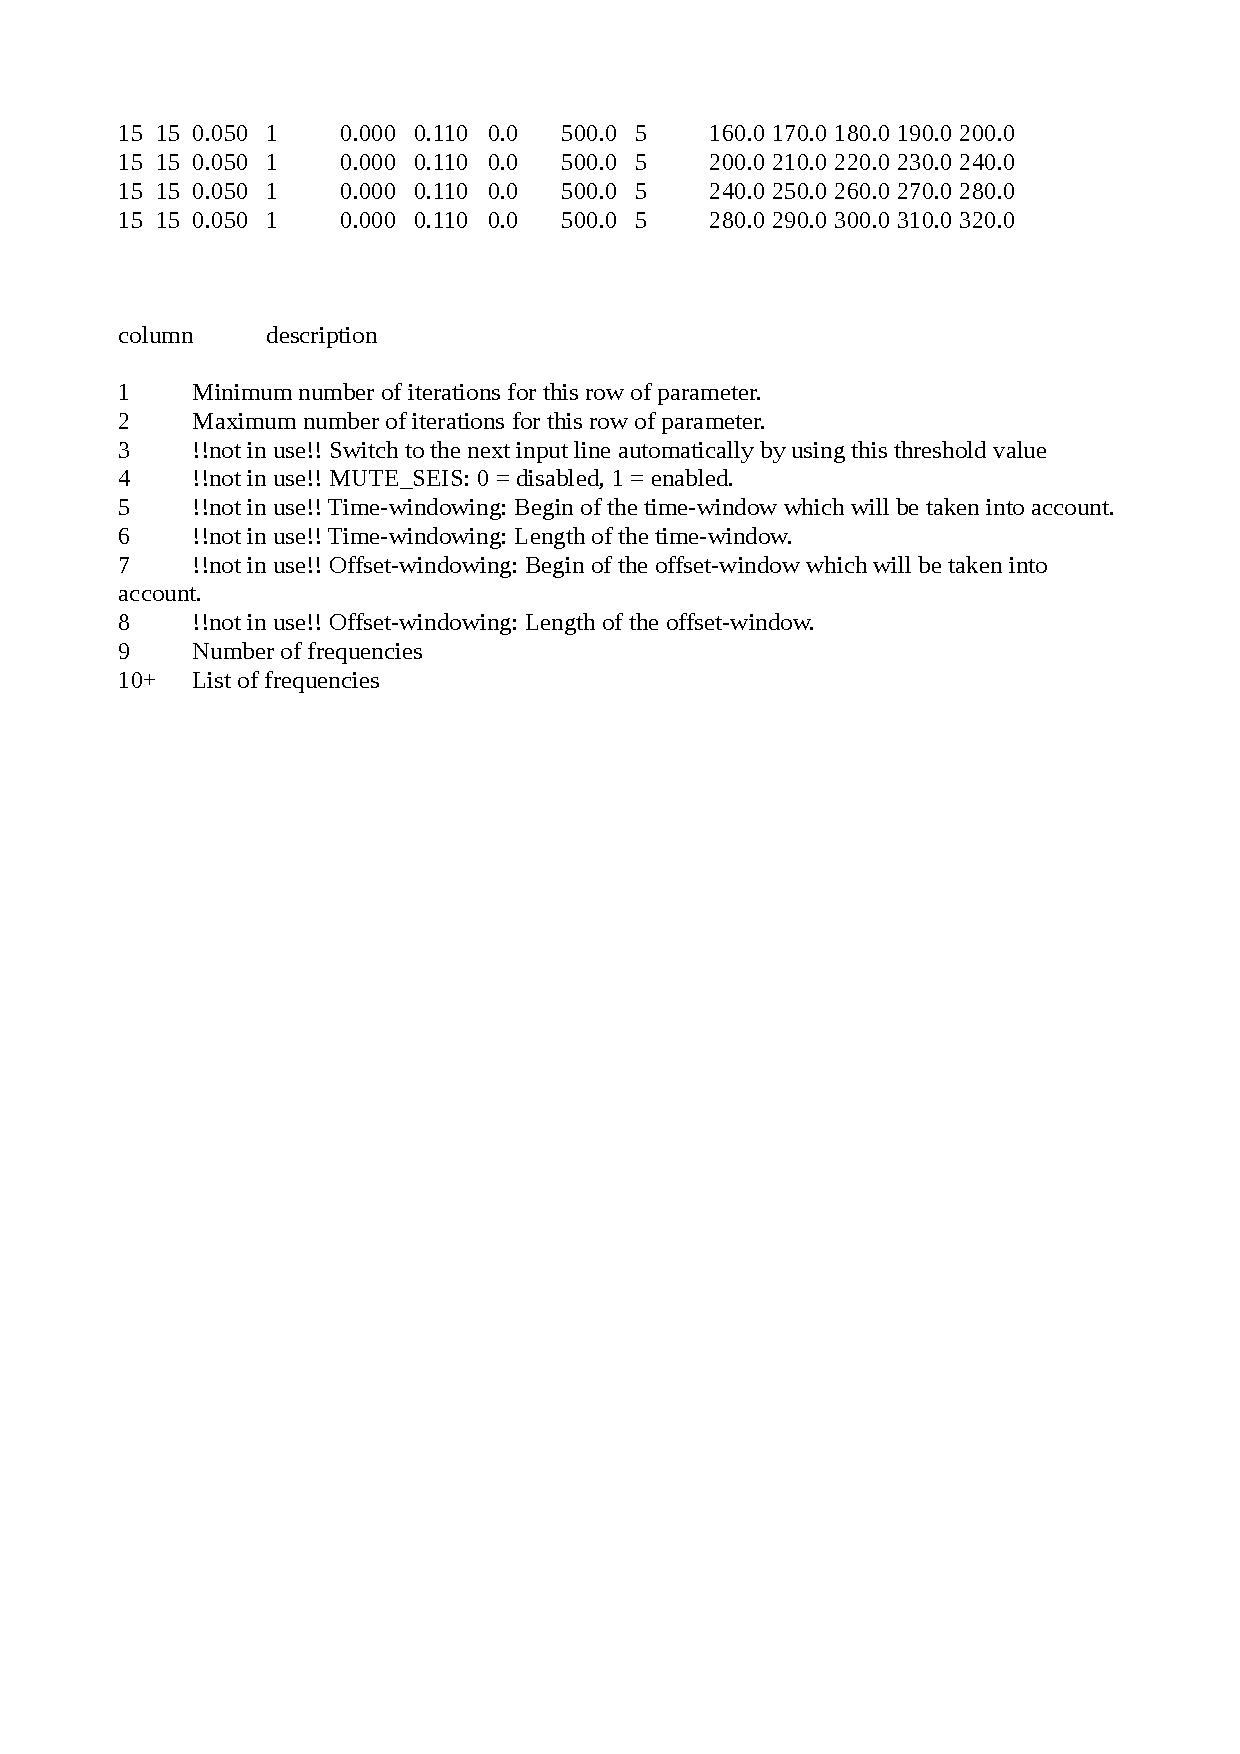
\includegraphics[width=\textwidth]{fig/workflow_input}
\caption[Workflow.dat]{The file workflow.dat organises the different inverion stages.}\label{fig:workflow_input}
\end{center}
\end{figure}
\subsection{Hessian}
\begin{verbatim}
"Hessian" : "comment",
			"HESS" : "0",
			"READ_HESS" : "0",
			"REC_HESS" : "1", 
			"WATER_HESS_VP, WATER_HESS_VS, WATER_HESS_RHO" : "0.0192, 0.0192, 1.0e-14",
			"HESS_FILE" : "./hess/toy_hess",
\end{verbatim}

If the option \textit{HESS}=1 is chosen in the input file, a diagonal Hessian approximation is applied for preconditioning of the gradients. If the Hessian approximation is already calculated it can be read from file (\textbf{READ\_HESS}=1). Hereby the hessian approximation is read from the folder \textit{hess}. The files written at the beginning of the current frequency stage are used, labeled for example \textit{hess/toy\_hess.vp\_200.00Hz\_it11} when the new frequency stage started with iteration 11. \\
For \textbf{READ\_HESS}=0 the diagonal Hessian approximation is calculated in IFOS3D as described in section~\ref{sec:hess}.\\
Due to runtime and storage it is recommendable to use only a subset of receivers for its calculation. The option \textbf{REC\_HESS} is not fully implemented at the moment, and it is therefore necessary to change the receiver file or the distance in the receiver array to its double or its triple value. \\
The water level (\textbf{WATER\_HESS}) used for the calculation of the preconditioning matrix (equation~\ref{Hess_precon}) can be estimated from the gradient of the first iteration and the diagonal Hessian matrix. It is not calculated directly in IFOS3D. This results in the fact, that it is not possible to perform a full inversion at a stretch, but the inversion needs to be split up into the different inversion stages.\\
The diagonal Hessian matrix is stored in the folder \textit{hess} and is labeled \\e.g. \textit{hess/toy\_hess.vp\_200.00Hz\_it11}. It is calculated at the beginning of each frequency stage and is applied within this frequency stage.
\subsection{L-BFGS}
\begin{verbatim}
"L-BFGS" : "comment",
			"LBFGS" : "0",
			"NUMPAR" : "2",
			"BFGSNUM" : "5"
\end{verbatim}

If \textbf{LBFGS}=1 the L-BFGS method is applied as described in section~\ref{sec:lbfgs}. The L-BFGS approach can only be used combined with the Hessian preconditioning (\textbf{HESS}=1). So far we tested the L-BFGS approach only for the seismic velocities, not for density. The number of inverted parameter classes (\textbf{NUMPAR}) can thus be chosen as 1 ($v_p$ only) or 2 ($v_p$ and $v_s$).\\
The L-BFGS algorithm estimates the Hessian from changes in gradients and models of the previous \textbf{BFGSNUM} iterations. 

\section{IFOS3D output}
\subsection{ifos3D.out}
The proceedings of the inversion can be followed in the file \textit{in\_and\_out/ifos3D.out} written by the first processor (MYID=0). This file gives information about parameters used in IFOS3D, grid dispersion and stability of the code. The proceedings of the forward modelings and output of the different sub-programs can be viewed. In case of an early termination of the program this file can be checked for an error message.
\subsection{ifos3D\_invers.out}
The output of misfit values and steplength information is written to \textit{in\_and\_out/ifos3D\_invers.out} during the run. The following values given for each iteration show the proceedings of the inversion:
\begin{itemize}
\item parameters as defined in the current iteration: the parameter \textbf{cdf} (set to one for the first iteration in each inversion stage), the lowest frequency used in this iteration and the number of frequencies for this stage. 
 \item misfit value (time domain) for each shot (\textbf{L2}), summed over shots (\textbf{L2all}) and misfit used for steplength calculation (\textbf{misfit[0]})
 \item test steplengths used for steplength estimation (\textbf{steplength}) and the resulting L2 misfits
 \item the steplength parabel and possible warnings given by \textit{src/steplength.c}
 \item the ''optimal`` steplength used for the model update and the estimated misfit for this steplength
 \item the new test steplength
\end{itemize}
If problems in the inversion occure this becomes generally quickly visible in its converge and in problems to find an optimum steplength.

